\documentclass[12pt]{article}\pagestyle{myheadings}

\title{Chord2Vec: Learning Chords Embeddings}
\author{Sephora Madjiheurem}
\usepackage[numbers]{natbib}
\usepackage{amsmath,amssymb,amsthm,amsfonts,graphics,subfigure,graphicx,enumerate,bbm} 
\usepackage[table,xcdraw]{xcolor}
\usepackage{tabularx,ctable,array}
\usepackage{natbib,caption}
\usepackage{algorithm,algpseudocode}
\usepackage{parnotes,float,multicol}
\usepackage{tikz}
\usetikzlibrary{positioning}
\newcolumntype{?}{!{\vrule width 1pt}}
\newcommand{\R}{\mathbb{R}}
\newcommand{\C}{\mathbb{C}} 
\newcommand{\N}{\mathcal{N}} 
\newcommand{\T}{\mathcal{T}}
\newcommand{\M}{\tilde{M}}
\newcommand{\tmij}{\tilde{m}_{ij}}
\newcommand{\mij}{{m}_{ij}}
\newcommand{\mjk}{{m}_{jk}}
\newcommand{\boldc}{\boldsymbol c}
\newcommand{\boldd}{\boldsymbol d}
\newcommand{\boldm}{\boldsymbol m}
\newcommand{\boldvd}{\boldsymbol v_d}
\newcommand{\boldve}{\boldsymbol v_e}
\newcommand{\boldvc}{\boldsymbol v_{c'}}
\newcommand{\boldvci}{\boldsymbol v_{c_{<i}}}
\DeclareMathOperator*{\argmin}{argmin}

\begin{document}
\maketitle

\section{Introduction}

The word2vec model by \citet{mik2013} allows to learn vector representations of words that carry syntactic and semantic meanings and that are useful in various natural language processing (NLP) tasks. In this work, we look at the similar problem on music data. Indeed, arbitrary encodings of polyphonic music provide no useful information regarding the relationships that may exist between the individual musical chords. The main goal of this study is to introduce techniques that can be used for learning high-quality embedding chord vectors from sequences of polyphonic music. 

We aim to achieve this by finding chord representations that are useful for predicting the neighboring chords in a musical piece. Formally, given a corpus of chords  $\T = \{\boldd_1, \boldd_2, \ldots, \boldd_T\}$ and the neighborhood of size $2j$ of a chord $\boldd_t$ defined by $ C(\boldd_t) = \{\boldd_{t+j}, -m \leq j \leq m , j \neq 0\}$, the objective is to maximize the average log probability with respect to some model parameters~$\theta$: 

\begin{equation}
\max_{\theta} \frac{1}{|\T|}\sum_{\boldd_t \in \T} \sum_{\boldc' \in C(\boldd_t)} \log p(\boldc = \boldc'|\boldd_t, \theta)
 \,.
\label{eq:c2v_obj}
\end{equation} 
In the remaining of this report, we will ease the reading by omitting the subscripts of the chords. Throughout this work, will consider a neigborhood window of size 2 (i.e. $j=1$).

We propose three different models inspired by model architectures used within the field of NLP. We train and evaluate each of these models on five different datasets. Finally we suggest directions for future work. 

\section*{Linear model}
Our first model is a naive adaptation of the Skip-gram model introduced by \citet{mik2013}. The main difference with the original Skip-gram model is that a text can be represented as a sequence of words, where each word can be represented as a ``one-hot" vector. In the case of music, we need a  ``many-hot" vector to represent a chord, as more than one note can be heard simultaneously. Hence, we replace the last softmax layer in Skip-gram by a sigmoid layer, to predict each note individually.  


The architecture of the first proposed model is shown in Figure~\ref{eq:c2v_obj}. It is a feed forward neural network that consists of input, hidden and output layers. At the input layer, a chord is encoded using a fixed length binary vector $\nolinebreak{\boldc = \{c_1, c_2, \ldots, c_N\}\in \{0,1\}^N}$, where $N$ is the number of notes in the vocabulary. In this chord representation, the entries that are set to $1$ correspond to the notes that are \textit{on} in the chord, whereas the notes that are \textit{off} are set to $0$. 

The weights between the input layer and the hidden layer can be represented by a matrix $M\in \R^{D \times N}$. Similarly, the weights between the hidden layer and the output layer can be represented by a matrix $\M\in \R^{N \times D}$. 

\begin{figure}[ht]
\centering 

\tikzset{%
   neuron missing/.style={
    draw=none, 
    scale=1.5,
    text height=0.333cm,
    execute at begin node=\color{black}$\vdots$
  },
}

\begin{tikzpicture}[x=1.3cm, y=.80cm, >=stealth]

\foreach \m [count=\y] in {1,2,3}
  \node [circle,fill=gray!50,minimum size=0.5cm ] (input-\m) at (0,2.5-\y) {};
  
\foreach \m [count=\y] in {4}
  \node [circle,fill=gray!50,minimum size=0.5cm ] (input-\m) at (0,-2.05) {};
  
 \node [neuron missing]  at (0,-1.2) {};

\foreach \m [count=\y] in {1}
  \node [circle,fill=gray!50,minimum size=0.5cm ] (hidden-\m) at (2,0.75) {};
  
\foreach \m [count=\y] in {2}
  \node [circle,fill=gray!50,minimum size=0.5cm ] (hidden-\m) at (2,-1.45) {};
  
 \node [neuron missing]  at (2,-0.3) {};

\foreach \m [count=\y] in {1,2,3}
  \node [circle,fill=gray!50,minimum size=0.5cm ] (output-\m) at (4,2.5-\y) {};
  
\foreach \m [count=\y] in {4}
  \node [circle,fill=gray!50,minimum size=0.5cm ] (output-\m) at (4,-2.05) {};
  
 \node [neuron missing]  at (4,-1.2) {};

\foreach \l [count=\i] in {1,2,3,N}
  \draw [<-] (input-\i) -- ++(-1,0)
    node [above, midway] {$d_{\l}$};

\foreach \l [count=\i] in {1,D}
  \node [above] at (hidden-\i.north) {$h_{\l}$};

\foreach \l [count=\i] in {1,2,3,N}
  \draw [->] (output-\i) -- ++(1,0)
    node [above, midway] {$c_{ \l}$};

\foreach \i in {1,...,4}
  \foreach \j in {1,...,2}
    \draw [->] (input-\i) -- (hidden-\j);

\foreach \i in {1,...,2}
  \foreach \j in {1,...,4}
    \draw [->] (hidden-\i) -- (output-\j);

\end{tikzpicture}
\caption{Linear model architecture}
\label{fig:lin-archi}
\end{figure}

The $D$-dimensional vector representation $\boldvd$ of the associated chord $\boldd$ is simply the normalized sum of the columns of $M$ that correspond to the notes occurring in chord $\boldd$:
\[ \boldvd = M\frac{ \boldd}{\| \boldd \|_1}
\]
To compute the probabilities in (\ref{eq:c2v_obj}) under this model, a  conditional independence assumption between the notes in a context chord $\boldc$ given a chord $\boldd$ is made, i.e 

\begin{equation}
p(\boldc =\boldc' | \boldd) = \prod_{i=1}^N  p(c_i =c_i'|  \boldd) \,.
\end{equation} 

\noindent Using weights matrices $M$ and $\M$, we define the scoring function $\nobreak{h: \mathcal{N}~\times~\mathcal{C}\mapsto\mathbb{R} :}$
\begin{equation}
h(i,\boldd) =  \M_{(:,i)} \boldvd \,,
\end{equation}
where $\M_{(:,i)}$ denotes the $i$'th row of $\M$.

\noindent
We then use the sigmoid function to model the conditional probabilities :
\begin{equation}
p(c_i =c_i'|  \boldd) = \left\{
                \begin{array}{lll}
                  \sigma\big( h(i,\boldd) \big) = \frac{\exp(h(i,\boldd))}{1 + \exp(h(i,\boldd))} & c_i' = 1 \\
                  1- \sigma\big( h(i,\boldd) \big) = \sigma\big( - h(i,\boldd) \big) = \frac{1}{1 + \exp(h(i,\boldd))} & c_i' = 0\\
                \end{array}
              \right.
\end{equation}

This model is not expected to perform well, mainly because of the independence assumption between the notes in a chord. In fact, it is very likely that there is a strong dependency between the notes appearing in a chord. In the next section, we introduce a model that does not make such an independence assumption and is therefore expected to lead to improved results. 

\section*{Autoregressive model}

The second proposed model is inspired by the The Neural Autoregressive Distribution Estimator (NADE) which allows to model the distribution of high-dimensional vectors of discrete variables \citep{larochelle2011}.

It decomposes the context chord probability distribution according to the chain rule as follows:

\begin{equation}
p(\boldc =\boldc' | \boldd) = \prod_{i=1}^N  p(c_i =c_i'|  \boldd, c_{<i}) \,,
\end{equation} 

where $c_{<i} = \{c_1, \ldots, c_{i-1}\}$.

Using weights matrices $M, L \in \R^{D \times N}$ and $W\in \R^{N \times D}$, we define a new scoring function $h$:

\begin{equation}
h(i,\boldd,c_{<i}) =  W_{:,i} \cdot (\boldvd + \boldvci) \,,
\end{equation}

where $\boldvci$ is defined as 
$ \sum_{j<i}  L_{:,j} c_j$.

We then use the scoring function to model the individual conditional probabilities: 

\begin{equation}
p(c_i =c_i'|  \boldd, c_{<i}) = \left\{
                \begin{array}{lll}
                  \sigma\big( W_{:,i} \cdot (\boldvd + \boldvci) \big)  & c_i' = 1 \\
                  1- \sigma\big( W_{:,i} \cdot (\boldvd + \boldvci) \big)  & c_i' = 0\\
                \end{array}
              \right.
\end{equation}

where $\boldvd = M\frac{ \boldd}{\| \boldd \|_1}$ is the D-dimensional vector representation of chord and $\sigma : \mathbb{R} \mapsto \mathbb{R}$ is the sigmoid function. 


\section*{Sequence-to-sequence model}

We propose to use another model to learn chord embeddings by learning which notes are compatible in a chord. This model is known as the sequence-to-sequence model \citep{SutskeverVL14}. In this setting, a chord is represented as a sequence of notes in some fixed ordering: $c \subseteq \N$, where $\N$ is the ordered set of all possible notes. Chord have arbitrary sizes. 


Sequence-to-sequence models allow to learn a mapping of input sequences of varying lengths to output sequences also of varying lengths. It uses a neural network architecture known as RNN Encoder-Decoder. Figure~\ref{fig:seq2seq} depicts the model architecture. 
\begin{figure}[ht]
\centering
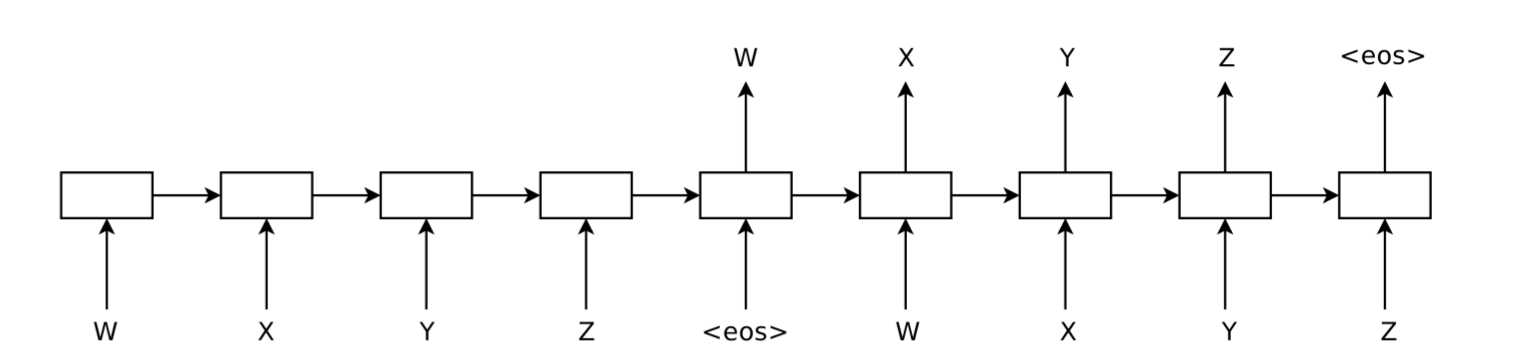
\includegraphics[width=1.0\linewidth]{figures/seq2seq.png}
\caption{\label{fig:seq2seq}Sequence-to-sequence (\citet{SutskeverVL14})}
\end{figure}
An LSTM encoder is used to map the input sequence to a fixed length vector, and another LSTM decoder is then used to extract the output sequence from this vector. The general goal is to estimate 
$
p(y_1,\ldots,y_{T'} | x_1, \ldots, x_T)\,,
$
where $x_1, \ldots, x_T$ and  $y_1,\ldots,y_{T'}$ are the input and output sequences respectively, and $T'$ and $T$ need not to be equal. 

The objective is given by:

\begin{equation}
\max_{\theta} \frac{1}{|\T|} \sum_{(X,Y) \in \T} \log p(Y|X,\theta) \,,
\label{eq:seq2seq_obj}
\end{equation}

where $Y$ is a correct output given the input $X$, $\T$ is the training set and $\theta$ is the set of the model parameters. 
The encoder and decoder are jointly trained to maximize the objective according to $\theta$.

The model estimates the conditional probability $p(y_1,\ldots,y_{T'} | x_1, \ldots, x_T)$ by first obtaining the fixed-length vector representation $v$ of the input sequence (given by the last state of the LSTM encoder) and then computing the probability of $y_1,\ldots,y_{T'} $ with the LSTM decoder: 

\begin{equation}
p(y_1,\ldots,y_{T'} | x_1, \ldots, x_T) = \prod_{t=1}^{T'} p(y_t|v, y_1,\ldots,y_{t-1})
\end{equation}

The sequence-to-sequence model can be used to learn embeddings for chords, by training the model to learn the context of a given chord. 

At the chord level, the encoder projects all notes in a chord into a joint note representation and a decoder generates all notes in a chord given a chord representation and previously generated notes.
 

The overall goal is to estimate
$
p(c_1, \ldots, c_T | d_1,\ldots,d_{T'})\,,
$
where  $d_1, \ldots, d_{T'}$ and $c_1, \ldots, c_T$ are in $\N$, $d = d_1, \ldots, d_{T'}$ is an input chord and $c_{t+j} =n^{(j)}_1, \ldots, n^{(j)}_T$ is a neighbor of $c$.

If $C(d)$ denotes the set of chords that are in the neighborhood of the chord $d$, then the objective in (\ref{eq:seq2seq_obj}) can be written as:

\begin{equation}
\max_{\theta} \frac{1}{|\T|} \sum_{d \in \T} \sum_{c\in C(d)} \sum_{t=1}^{|c|} \log p(c_t | v_d, c_1, \ldots, c_{t-1})  \,,
\label{eq:c2c_obj}
\end{equation}

where $v_d$ is the vector representation of the input chord $d$. 

\section*{Experiments }

\subsubsection*{Data sets}
We compare the performance of the different models on five datasets of varying complexity:

\begin{itemize}
\item[] \textbf{JSB Chorales}: corpus of 382 four-part harmonized chorales by J.S. Bach with the split of  \citet{allan2005harmonising}
\item[] \textbf{Nottingham}: collection of 1200 folk tunes with chords instantiated from the ABC format
\item[] \textbf{MuseData}: electronic library of orchestral and piano classical music from CCARH
\item[] \textbf{Piano-midi.de}: classical piano MIDI archive split according to \citet{poliner2007discriminative}
\item[] \textbf{Mix}: a collection of all above datasets.
\end{itemize}

\noindent In these data sets, the polyphony varies from 0 to 15 and the average number of simultaneous notes is $3.9$. The range of notes spans the whole range of piano from A0 to C8, i.e. $N = |\N| = 88$.
The the training data was augmented as follows: we transpose each piece by $\phi$ semi-tones, for $\phi = -6, -5, . . . , 4, 5.$
\\

\subsubsection*{Baseline models}

In addition to the previously mentioned models, we compare our results with the two following methods:
 \begin{itemize}
 \item \textbf{Random}: the simplest baseline simply models the probability distribution of each note by the uniform probability distribution, i.e. $$p(c_i = c_i' | d ) = 0.5$$.
 \item \textbf{Marginal distribution}: the second model computes the marginal probability distribution of the notes in the training data: $$p(c_i = 1 | d )= \frac{z_i + \alpha}{|\T|+\alpha} ,$$ where $z_i$ is the number of the occurrences of note $i$ in the training set $\T$ and $\alpha = 1$ is the constant used for additive smoothing.  
 \end{itemize}

\subsubsection*{Implementation Details}
The linear chord2vec model and the autoregressive chord2vec were trained in batches of size 128 with  Adam Optimizer using $D = 1024$. Each model is optimized for 200 epochs, but the final model is the one leading to the lowest validation error.  

Our sequence-to-sequence model architecture is a multi-layer LSTM cells with 2 layers with 512 units. To allow sequences of varying length, bucketing and padding methods are used. We append to each target chord an end-of-sequence symbol.

We implemented all three models using Google's Tensorflow library.

\section*{Results}

The negative log likelihoods on the test data for all models and on all data sets are presented in Table~\ref{tab:results}. First, we observe that our simple linear model, despite the independence assumptions, is able to actually learn something beyond the marginal distribution of the training set. Secondly, as expected, we observe that the autoregressive model achieves better scores than the simple linear model on all data sets, confirming our hypothesis that the notes in a chord are not independent of each other. Lastly, it appears that the Sequence-to-Sequence model is the model that leads to the lowest error overall.   

\begin{table}[ht]
\centering
\caption{Negative log likelihood on test data}
\begin{tabular}{l?lllll}
\hline
Model   & JSB Chorales & Nottingham & MuseData & Piano-midi.de & Mix \\ \hline
Random & 60.9969 & 60.9970 & 60.9970 & 60.9970 & 60.9972\\ 
Marginal & 12.2349 & 10.4449 & 23.7489 & 17.3590 & 15.2652 \\ 
Linear c2v & 9.7734 & 5.7609 & 15.4104&12.6835 & 12.1712  \\ 
Autoreg. c2v & 6.1853 & 3.9801 &14.4912 & 10.1847 & 7.4215 \\ 
Seq2Seq c2v & 1.1090 &  0.4974 & 1.5243 & 1.7795 & 1.2207 
\label{tab:results}
\end{tabular}
\end{table}

\section*{Future work}
Our study has revealed that the Sequence-to-Sequence model, which is the model with the most complex architecture, leads to the highest log likelihood on all five datasets. However, in the case of text classification problems, it has been shown that a simpler architecture can lead to results that are comparable to deep learning models in terms of accuracy and are much faster for training and evaluation \citep{JoulinGBM16}.
With this in mind, we introduce in this section as potential future work yet another model based on the Skip-gram model \citep{mik2013}.

We also suggest some directions for measuring the quality of the learned embedding vectors.

\subsection*{One more chord2vec model}
Although the architecture of the linear chord2vec model resembles the original Skip-gram's architecture  \citep{mik2013}, the following model seems to be a more direct adaptation of word2vec to chord2vec:
\begin{equation}
p(\boldc = \boldc'| \boldd) = \frac{\exp(\tilde{\boldvc} \cdot \boldvd)}{\sum_{\boldsymbol e \in \{0,1\}^N } \exp(\tilde{\boldve} \cdot \boldvd)} \, \,
\end{equation}

where $\boldvd = M\frac{ \boldd}{\| \boldd \|_1}$ and $ \tilde{\boldvc} = \M \frac{ \boldc'}{\| \boldc' \|_1}$.


\noindent With this model, learning the vectors $\tilde{\boldsymbol v}_c$ is very expensive since we need to iterate through every possible chord. One solution to this scalability problem is to use \textit{noise-contrastive estimation} \citep{NIPS2013_5165}.  

Because this model does not make an assumption of independence between the notes occurring in a chord and given the success of the Skip-gram model for learning words embeddings \citep{mik2013}, one can expect such a model to perform well.


\subsection*{Evaluating the Learned Embeddings}
After having decided on the model leading to the lowest error on the test data, one could visualize the learned vectors by performing a dimensionality reduction using t-SNE or PCA for instance. An inspection of such low dimension vectors could help understanding whether the embedding vectors capture useful information about chords and their relationship to one anther. 

\bibliographystyle{plainnat}
\bibliography{bibli.bib} 
\end{document}